\documentclass[12pt, letterpaper]{article}
\usepackage[utf8]{inputenc}
\usepackage[document]{ragged2e}
\usepackage{graphicx}
\usepackage{comment}
\usepackage[normalem]{ulem} % for strikethrough text
\usepackage{float} % for passing float parameter into the picture environment

\graphicspath{{images/}}


% from here content will be shown
\begin{document}

\begin{titlepage}
\centering
{\Large DESIGN DOCUMENT} \\
\begin{figure}[h]
\centering

\includegraphics[width=5cm]{Logo_Politecnico_Milano.png}
\caption{Politecnico di Milano}
\label{fig:PoliMi}
\end{figure}
\textbf{version 1.0} \\
\vspace{0.5cm}
Artemiy Frolov, mat. 876373 \\
\vspace{0.5cm}
autumn 2016
\end{titlepage}


\tableofcontents{}

\newpage

\section{Introduction}
\subsection{Purpose}

The purpose of this document is to provide more technical details about the CarSharing System software application 

This document is directed to developers and is necessary to state these aspects of the developing system: 
\begin{itemize}
	\item high level architecture 
	\item runtime view 
	\item choosed architectural styles and patterns
	\item algorithm design of key components 
	\item possibly include some extensions of the user interface defined in RASD 
\end{itemize}

\subsection{Scope}

CarSharing is a web-based software application that helps car-sharing companies to increase usability of their service, by providing more convenient way of renting electric cars for clients via smartphones, hence helping clients to use the service in a more comfortable way. Thus, the software is targed only to:
\begin{itemize}
	\item Users
\end{itemize}    

System allow clients(Users) to locate available electrical cars, with all relevant information about it (inluding current battery fulness, address, registered number) nearby or in the specific area. \\ 
After selecting the car, user can reserve it for up to one hour. When a user reaches the reserved car, system allows the user to unlock the car via button in the web-app. As soon as the engine ignites, the system confirms that the car is now occupied and user can see current charges through the screen in
the car. \\
User can leave the car for a short period of time without missing the car occupation. When the user is no more needs the car, he presses the "Stop the trip" button, system locks the car and collect the money from the bank account, provided by user during registration. From this point the car is no more controlled by the user no more and it be becomes available again. \\
System, in order to restrain the behaviour of users, and to encourage virtuous behaviours of users, carries out some reward and punishment features.
Also the system uses external web-services to present the location of cars and to manage payments.   

\subsection{Definitions, Acronyms, Abbreviations}

\begin{itemize}
	\item RASD: requirement analysis and specification document 
	\item DD: design document
	\item SMS: short message service; used to notify users 15 minutes before the reservation time expires, also used for a short period suspendance warning. A SMS gateway is needed to use it.
	\item SMS gateway: it is a service which allows to send SMS via standard API.
	\item MVC: model view controller.
	\item URL: uniform resource locator
	%\item 
\end{itemize}


\subsection{Reference Documents} 

\begin{itemize}
	\item RASD produced before 1.1
	\item Specification Document: Assignments 1 and 2 (RASD and DD).pdf
\end{itemize}

\subsection{Document Structure}

\begin{itemize}
\item Introduction
	\begin{itemize}
		\item Purpose 
		\item Scope
		\item Definitions, Acronyms, Abbreviations
		\item Reference Documents
		\item Document Structure 
	\end{itemize}
\item Architecture Design
	\begin{itemize}
		\item Overview:	High level components and their interaction
		\item Component view
		\item Deployment view
		\item Runtime view: mostly contain sequence diagrams to describe the way components interact
		\item Component	interfaces
		\item Selected architectural styles and	patterns 
		\item Other	design decisions
	\end{itemize}
\item Algorithm Design
\item User Interface Design
\item Requirement Tracebility
\item Effort Spent
\item Reference

\end{itemize}

\newpage
\section{Architectural Design} 
\subsection{Overview}

The CarSharing system would have 3 tier client-server architecture. 

\begin{figure}[h]
\centering
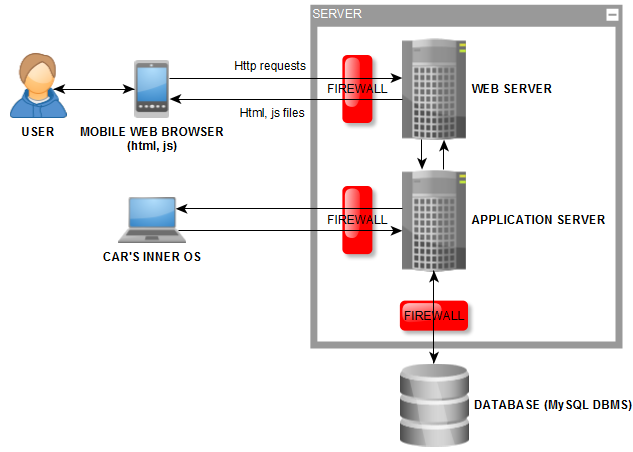
\includegraphics[width=\textwidth]{hlarch.png}
\caption{High-level architecture representation}
\label{fig:hlarch}
\end{figure}

\textbf{Mobile web browser:} browser that user uses on his/her smartphone. \\ 
\textbf{Web server:} Server that processes http requests. \\
Mobile web browser sends http requests to the web server, which responds by sending proper html and js files. \\
Mobile web browser and web server form the GUI and both correspond to the Presentation tier of the cliet-server high-level architecture. \\
\vspace{0.5cm}
\textbf{Application server:} server that processes the data and manage application logic. \\ 
Application server corresponds to the Logic tier of the cliet-server high-level architecture. \\
\vspace{0.5cm}
\textbf{Car's inner OS:} operating system of the electrical car. \\ 
\textbf{Database:} Persistent data storage. Implemented as DBMS. \\
Database corresponds to the Data tier of the cliet-server high-level architecture. \\
\vspace{0.5cm}
Application server receives user's activity information from the web server via RESTful API. Received information is then processed and can be stored in database or/and affect electrical car states. \\
Application server communicates with the electrical car's inner OS via 3G.\\
\vspace{0.5cm}
Moreover each tier is strongly secured with firewalls to avoid illegal system breaches.

\subsection{High level components and their interactions}

\begin{figure}[h]
\centering
\includegraphics[width=\textwidth]{hlcomponents.png}
\caption{High-level components}
\label{fig:hlcomp}
\end{figure}

\subsection{Component view}

\begin{figure}[h]
\centering
\includegraphics[width=\textwidth]{componentview.png} % ToDo
\caption{Components View}
\label{fig:compview}
\end{figure}

\begin{itemize}
	\item RequestController: manages the incomming http requests from users and redirect them to system services.
	\item RegistrationController: maintains collected registration information, incuding checking validity of inputed data. 
	\item LogInController: checks if user and password exist in database. 
	\item Reservationontroller: manages car reservation. The most important part of the system. It: 
	\begin{itemize}
	   	\item updates reservation status of the car in database.
	   	\item includes backward timer that restricts the time of car reservation during "reserved" status and suspended car during "occupied" status. It provides time to NotificationController.  
	   	\item communicates with LocationController(and implicitly with Car) to activate page car control buttons in user's browser.
	   	\item activates PaymentCalculator to sum up the cost of the ride. 
	\end{itemize}   
	\item NotificationController: sends warning messages to the user about soon expire time of reservation or time of car being suspended via SMS. Has access to the database to acquire telephone number of the user.
	\item LocationController: compares user's and car's locations to enable car controlling features. Communicates with CarController(and implicitly with the Car) to acquire GPS data of the car. Have access to database to acquire general information about the car.  
	\item CarController: Acquires information of the car from sensors, GPS and other relevant information for the CarSharing system. Sends request to the car for manipulation. 
	\item PaymentCalculator: sum up the cost of the ride. Sends requests to the CarController to collect sensors information. Collected information is then transformed into charges and discount of the ride. Has access to the database to collect payment information of the user. Uses external payment web services, sends requests to it with the amount of payment to take and address of the charged bank account. 
\end{itemize}

\subsubsection{Deployment View} 
\newpage
\subsection{Runtime view}
\subsubsection{Defining area of car search}
\begin{figure}[H]
\centering
\includegraphics[width=\textwidth]{3DefAreaOfSearch.png} % ToDo
\label{fig:3DefAreaOfSearch}
\end{figure}
\newpage
Firstly user chooses where to search cars: nearby user or nearby the specific area provided by user. In the diagram \ref{fig:3DefAreaOfSearch} at the beggining user either presses the button "Nearby" or he/she inputs address into the "Specific area" field and presses button "Submit". In both cases in the diagram these actions are treated as "User\_desired\_area\_of\_car\_search(coord)" and in both cases browser sends coordinates. \\
Then coordinates are transferred to the CarController, which compares coordinates with each car in the database. It also collects current information about the car, including battery fulness.  If car is not further than 3 (km\^2) from the coordinates it is added to the set of cars\_nearby. Proccess repeats until all cars are checked. \\
Then the set of cars\_nearby is sent to external map web service, which is placed in the web page.  
\newpage
\subsubsection{Choose the car}
\begin{figure}[H]
\centering
\includegraphics[width=\textwidth]{4ChooseCar.png} % ToDo
\label{fig:4ChooseCar}
\end{figure}
\newpage
When user presses on the car on the map the information about it appears near the map window and "reserve" button popes up. When after selecting the car user presses the button "reserve" the system checks the up-to-date information about that car if it is already reserved. If it is not reserved system reserves it for the user(updates the database) and showes the Reservation page.  
\newpage
\subsubsection{Car Is Reserved \#1}
\begin{figure}[H]
\centering
\includegraphics[width=\textwidth]{5CarIsReserved1.png} % ToDo
\label{fig:5CarIsReserved1}
\end{figure}
\newpage
After user reserved the car BackwardTimer is set to 1 hour. Until the timer is not equals to 0 the user can still occupy the car. When user presses the "unlock button" on the web page system checkes whether user is close to the car. If not it return the message "too far from the car to unlock". When users coordinates are close to the coordinates of the car and user presses the "unlock button" the system send request to the car to unlock itself. At this point when user enters the car and starts the engine, Car sends acknowledgement to the system, ReservationController changes car status to the "occupied", kills the timer and requests the webpage to show the occupation page. \\ 
Note: If the user once unlocked the car, being close to the car, the new validated button "lock" button can be used from any distance. \\
\newpage
\subsubsection{Car Is Reserved \#2 (continue)}
\begin{figure}[H]
\centering
\includegraphics[width=\textwidth]{6CarIsReserved2.png} % ToDo
\label{fig:6CarIsReserved2}
\end{figure}
\newpage
If the timer is went to zero and user haven't started the engine, the system changes car status to "available" and asks the PaymentCalculator to sum up the cost, providing the charge of 1 euro. The error message "reservation is expired" appears in the browser and after few seconds main page is shown.  \\
In the diagram \ref{fig:6CarIsReserved2} the frame "Payment" describes the basic algorithm of the PaymentCalculator. If the addit\_arg is equals to "null", than the algorithm describes the case, when user stoppes the trip by himself and the step 6 can be ommitted. \\
In order to restrict the situation when user get into the car, but timer went to 0, system blocks and suspends(if user catched to start it) the car starter and locks the car(not seen in the diagram \ref{fig:6CarIsReserved2}). In that case user can unlock the door from inside, walk off the car and it will automatically lock it again.
\newpage
\subsubsection{Car Is Occupied}
The runtime diagram is redundant to describe that moment of system use as it doesn't have any new specific cases that haven't been described yet and mechanisms of implementation are the same.
Brief description:
\begin{itemize}
	\item System provides the "Occupied" page, which contains 2 buttons - "lock/unlock" and "End of the Trip"
	\item Procedure of using buttons "lock/unlock" has been described in the runtime diagram \ref{fig:5CarIsReserved1} from the beggining.
	\item Button "End of the Trip" simply sends request to the ReservationController to change car status to "available". After that ReservationController sends request to the CarController to block the car starter(Car also locks itself) and requests the PaymentCalculator to sum up the total cost of the ride(see diagram \ref{fig:6CarIsReserved2} and read the description below).
\end{itemize}  
\newpage













\newpage
\section {Effort Spent} 
\textbf{Artemiy Frolov:}
\begin{verbatim}
26/11, 1h
28/11, 0.5h
30/11, 3h
1/12, 3h
2/12, 2h
3/12, 3h
4/12, 4h
\end{verbatim} 

\newpage
% INTRODUCTION END

\end{document}